_
\documentclass[10pt]{beamer}

\usetheme{CambridgeUS}
\usepackage[english, russian]{babel}
\usepackage[utf8]{inputenc}
\usepackage{caption}
\usepackage{etoolbox}
\usepackage{multicol}
\usepackage{listings}
\usepackage{color}

\definecolor{mygreen}{rgb}{0,0.6,0}
\lstset{
  basicstyle=\ttfamily\footnotesize,        % the size of the fonts that are used for the code
  breaklines=true,                 % automatic line breaking only at whitespace
  captionpos=b,                    % sets the caption-position to bottom
  commentstyle=\color{mygreen},    % comment style
  keywordstyle=\color{blue},       % keyword style
  stringstyle=\color{red},     % string literal style
  showstringspaces=false,
  morekeywords={include, printf},
  texcl=true     %<---- added
  numbersep=14pt
}

\title[\href{https://goo.gl/NRgp8K}{https://goo.gl/NRgp8K} (Term 3)]{Точки следования, UB, sizeof, inline, ?: }
\author[Зацепин Михаил]{Зацепин Михаил}
\institute[МФТИ] 
{Московский физико-технический институт\\*}
\date{Москва, 2018}
\subject{Computer Science}

\begin{document}

\begin{frame}
  \titlepage
\end{frame}

\section{Точки следования (пример)}
\begin{frame}[fragile]{Затравка}
\begin{lstlisting}[language=C++]
    i = ++i + i++;
\end{lstlisting}
    \pause
\begin{lstlisting}[language=C++]
    f(++i, ++i);
\end{lstlisting}
    \pause
\begin{lstlisting}[language=C++]
    a[i] = i++;
\end{lstlisting}
\end{frame}

\section{UB и компания}
\begin{frame}{UB и компания}
\begin{itemize}
\item{\texttt{ill-formed} - диагностика на этапе компиляции}
\item{\texttt{implementation-defined behavior} - поведение зависит от реализации, но должно быть документировано (\texttt{std::size\_t})}
\item{\texttt{unspecified behavior} - зависит от реализации, не обязано быть задокументировано, любой из вариантов валиден}
\item{\texttt{undefined behavior} - нет ограничения на поведение программы (выход за пределы массива)}
\end{itemize}
\end{frame}

\section{Точки следования (до C++11)}
\begin{frame}{Side effects}
\begin{itemize}
\item{Модификация объектов}
\item{Вызов функций ввода-вывода}
\item{Вызов функций, которые модифицируют объект и т.д.}
\end{itemize}
\end{frame}

\section{Точки следования (до C++11)}
\begin{frame}{Точка следования (Sequence Point)}
\textcolor{red}{Точка следования} - это точка последовательности выполнения, в которой все побочные эффекты от вычислений, стоящих раньше в последовательности, завершены, и никакие побочные эффекты, относящиеся к последующим вычислениям, не начали выполнятся.
\end{frame}

\section{Точки следования (до C++11)}
\begin{frame}[fragile]{Точка следования (Sequence Point)}
Правила:
\begin{itemize}
\item{Точка следования находится в конце каждого полного выражения (обычно, она расположена на точке с запятой)}
\item{При вызове функции (включая \texttt{inline}) точка следования находится после вычисления всех аргументов функции (если таковые имеются), которое происходит перед выполнением любых выражений или инструкций в теле функции.}
\item{Точка следования находится после копирования возвращаемого значения функции и перед выполнением любых выражений за пределами функции}
\item{Выполнение функций не может чередоваться}
\item{Операторы:}
\end{itemize}
\begin{lstlisting}[language=C++]
    a && b
    a || b
    a ? b : c
    a, b
\end{lstlisting}
\end{frame}

\section{Undefined Behavior}
\begin{frame}[fragile]{Неопределенное поведение}
Между точками следования, значение скалярного объекта не должно изменяться более одного раза
\begin{lstlisting}[language=C++]
i = ++i + i++;
f(++i, ++i);
\end{lstlisting}
\pause
Между точками следования, предыдущее значение скалярного объекта, которое модифицировано при вычислении выражения, должно быть доступно только для определения сохраняемого значения
\begin{lstlisting}[language=C++]
 a[i] = i++;
\end{lstlisting}
\end{frame}

\section{Точки следования (с C++17)}
\begin{frame}[fragile]{Отношение sequenced-before}
Вместо Sequence Points - отношение \textcolor{red}{sequenced-before}
\begin{lstlisting}[language=C++]
a.b
a->b
a->*b
a(b1, b2, b3)
b @= a
a[b]
a << b
a >> b
\end{lstlisting}
\end{frame}

\section{Зачем это иметь в виду?}
\begin{frame}[fragile]{Отношение sequenced-before}
\begin{itemize}
\item{Что-то осталось \texttt{Undefined}}
\item{Поддержка \texttt{C++17} компиляторами}
\end{itemize}
\pause
\begin{lstlisting}[language=C++]
void f()
{
  std::string s = "but I have heard it works even if you don’t believe in it";
  s.replace(0, 4, "").replace(s.find("even"), 4, "only").replace(s.find(" don't"), 6, "");
  assert(s == "I have heard it works only if you believe in it");
}
\end{lstlisting}
\end{frame}

\section{sizeof}
\begin{frame}[fragile]{оператор sizeof}
\begin{itemize}
\item{Результат на этапе компиляции, то есть выражение \textcolor{red}{не вычисляется}!}
\item{Возвращает значение типа \texttt{std::size\_t}}
\end{itemize}
Синтаксис:
\begin{itemize}
\item{\texttt{sizeof( type )}}
\item{\texttt{sizeof expression}}
\end{itemize}
\end{frame}

\section{Размеры типов}
\begin{frame}[fragile]{Размеры типов}
\begin{itemize}
\item{\textt{[unsigned|signed] sizeof(char)} == 1}
\pause
\item{Кол-во бит в \textt{char} задается в константе \textt{CHAR\_BIT}. Обычно 8, но это неточно}
\end{itemize}
\end{frame}

\section{Размеры типов}
\begin{frame}[fragile]{Размеры типов}
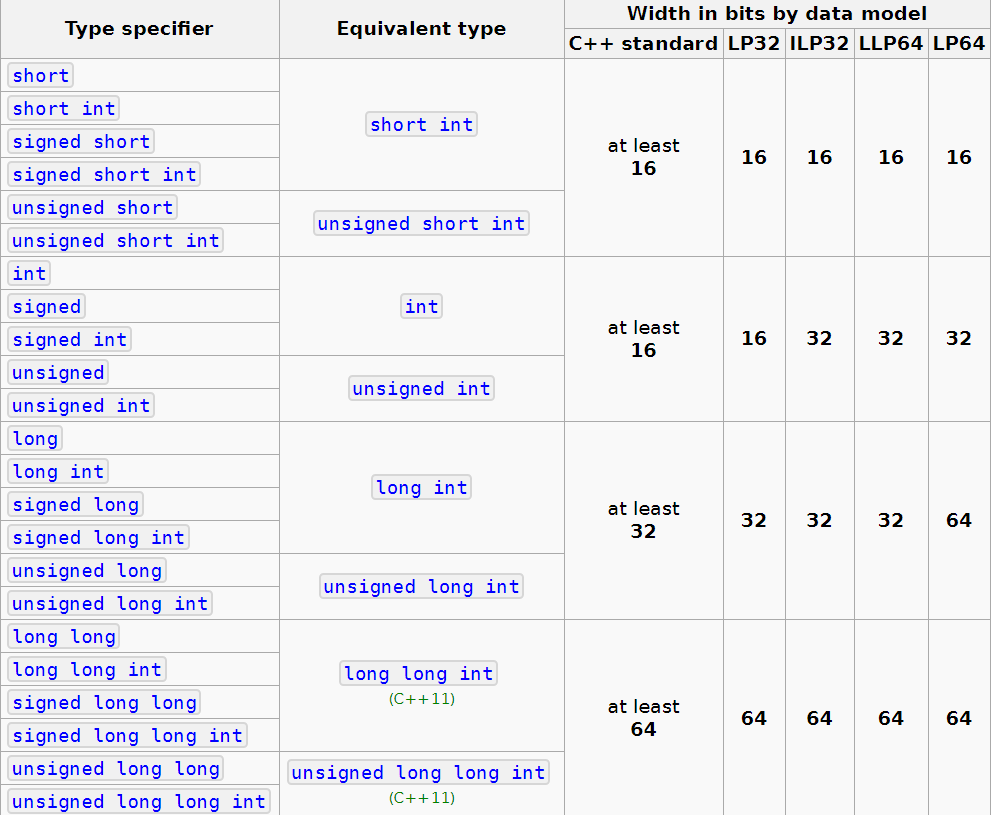
\includegraphics[scale=0.35]{Term_3/Source/Pictures/TypesRanges.png}
\end{frame}

\section{Размеры типов}
\begin{frame}[fragile]{Размеры типов}
Гарантируется лишь, что:
\begin{lstlisting}[language=C++]
1 == sizeof(char) <= sizeof(short) <= sizeof(int) <= sizeof(long) <= sizeof(long long)
\end{lstlisting}
\pause
Поэтому возможна ситуация, когда все типы по 64 бита, и \textt{sizeof} всегда возвращает 1
\end{frame}

\end{document}